\section*{Results}

Measuring the success of a hack week objectively is complicated by the variety of objectives that a hack week might have (see above).
Additionally, the participant-driven, open-ended format facilitates knowledge transfer and collaborations in sometimes surprising ways that escape traditional measures of success.
One key metric is the number of publications that result from hack week projects, but this is a fairly narrow definition of success, in line with standard academic performance indicators.
Assuming that participants work largely in the open during a hack week, and that most projects have a strong programming component another indicator of success is the activity of participants in terms of code written and committed to a public code repository.
Still, these measures ignore learning, community-building as well as networking outcomes.
These outcomes can be assessed through post-workshop surveys.
%It is in principle possible to measure gains in knowledge, networks and productivity within the pool of acceptable candidates for both those that attended the hack week and those that did not.
%This would then provide a somewhat objective measure of the impact the hack week has had.
%In practice, this has not been done for any of the hack weeks conducted thus far.
Here, we have taken an approach that combines these metrics: we start with survey results, and anecdotally report about publications, new code and projects generated (see \ref{box:outcomes})
%Open-ended questions allow participants to provide feedback about outcomes, problems and goals that organizers had not anticipated.

%If hack week organizers plan to conduct research that involves hack week participants (for example, using assessments and evaluations in a paper such as this one) it is important to obtain approval from the Institutional Review Board (IRB), or equivalent body that approves research with human participants at the institution hosting the hack week.
%Though this research would usually fall under the category of ''minimal risk``, it is still important to establish procedures to manage these data, and to obtain informed consent.
%In particular, in some cases hack week organizers may be interested in studying not only the participants in the hack week, but also the applicants who did not end up participating.
%It is important to establish procedures to conduct such studies and to obtain approval from an IRB.

We report the outcomes of astro-, geo- and neuro- hack weeks from 2016. In the results from post-workshop surveys (collected with the approval of the Institutional Review Boards at UW, NYU and UC Berkeley, and with participants' informed consent), we focus on attitudes towards open science and reproducibility, their own learning outcomes, as well as community building and collaborations.

We find that at all three hack weeks, participant self-report successful learning outcomes in new topics, tools or methods (AHW: 86\%, GHW: 94\%, NHW: 76\% for responses ''somewhat agree``, ''agree`` and ''strongly agree``; Figure 2, left panel).
The overwhelming majority of respondents at the hack weeks ($>95\%$ for all three events) believed that they learned things that improve their day-to-day research, and that attendance has made them a better scientist (see Figure 2, middle and right panels).
%While each hack week also probed participants' attitudes in more detail toward specific topics, methods, and modes of learning, the hack weeks differed substantially on that level, making the results difficult to compare.
%Another important goal of the hack weeks was centred on community building and fostering collaborations.
We find that overall, the majority of participants felt that their contributions to their hack teams was valued, and that they built valuable connections to other researchers (Figure 3, middle panel).
This is especially true for Neuro Hack Week, where more than 64\% of participants strongly agreed that they formed valuable connections at NHW (Figure 3, right panel).
Because peer learning is a major mode of knowledge transfer at hack weeks, we asked participants whether they taught other participants.
We find that again a majority agrees with this statement to some degree (AHW: 83\%, GHW: 69\%, NHW: 71\% for combined responses ''somewhat agree``, ''agree`` and ''strongly agree``; Figure 3, left panel), though responses are not as unequivocal as they are in some of the other categories.
This is expected: participants new to the field may participate to learn rather than to teach.

Reproducibility and open science have recently drawn much attention from the scientific community, and all three hack weeks have been working to promote positive attitudes towards reproducibility and open science in their respective fields.
We find that hack weeks have been largely successful at encouraging open science: at all three events, more than 70\% of all participants (AHW: 79\%, GHW: 72\%, NHW:85\%; Figure 4, left panel) put code or data created at the hack week into a public repository, while a substantially smaller fraction of participants followed this practice before the event (Figure 4, middle panel).
When asking participants whether they had made their code or data openly available in the past, the overall behaviour reflects how general conventions and attitudes differ in different fields.
In particular, astronomy shows the largest degree of openness toward open science, whereas our results indicate that open science is still fairly uncommon in the geosciences, with neuroscience falling in between.
%Neuroscience seems to fall somewhere in between.
This implies that hack weeks can have the highest impacts in field where a priori engagement in reproducibility efforts is low and significant progress can be made towards changing researchers' attitudes during a collaborative workshop.
Similar attitudes are reflected when asking whether the hack week has made participants more comfortable with open science: again, geoscience shows the large improvement with over 97\% agreeing with this statement to some degree, closely followed by neuroscience (95\%), while there was somewhat less of an impact on participants' attitudes in astronomy (72\%).
Overall, our results show that hack weeks are effective at addressing persisting doubts about making research open and reproducible.

\begin{figure}[htbp]
\begin{center}
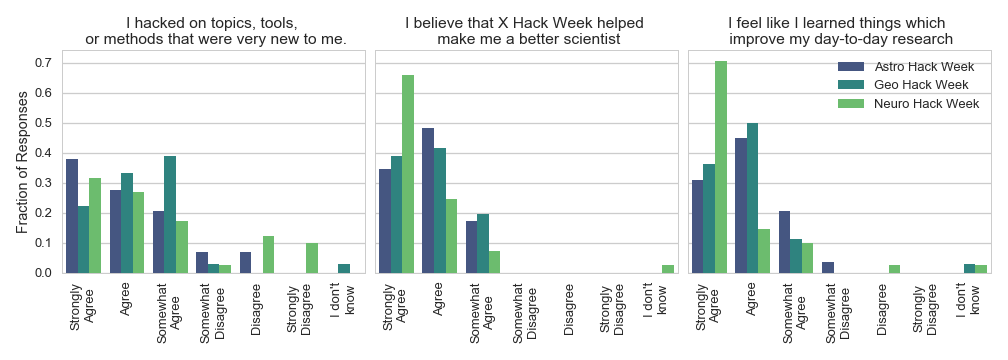
\includegraphics[width=12cm]{fig/eval_techskills}
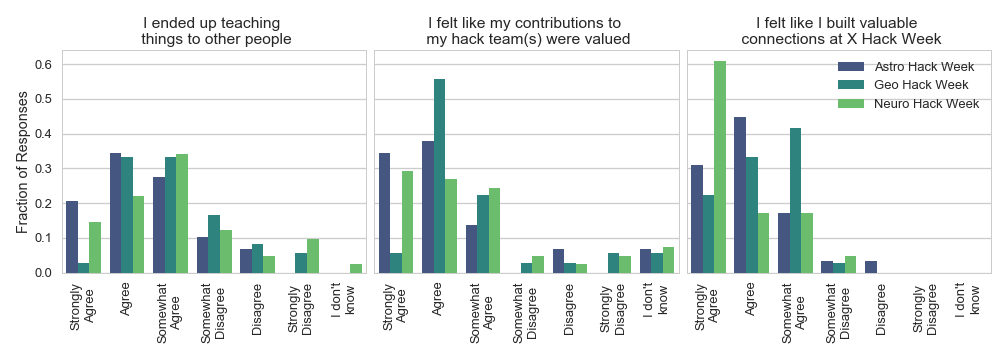
\includegraphics[width=12cm]{fig/eval_collab}
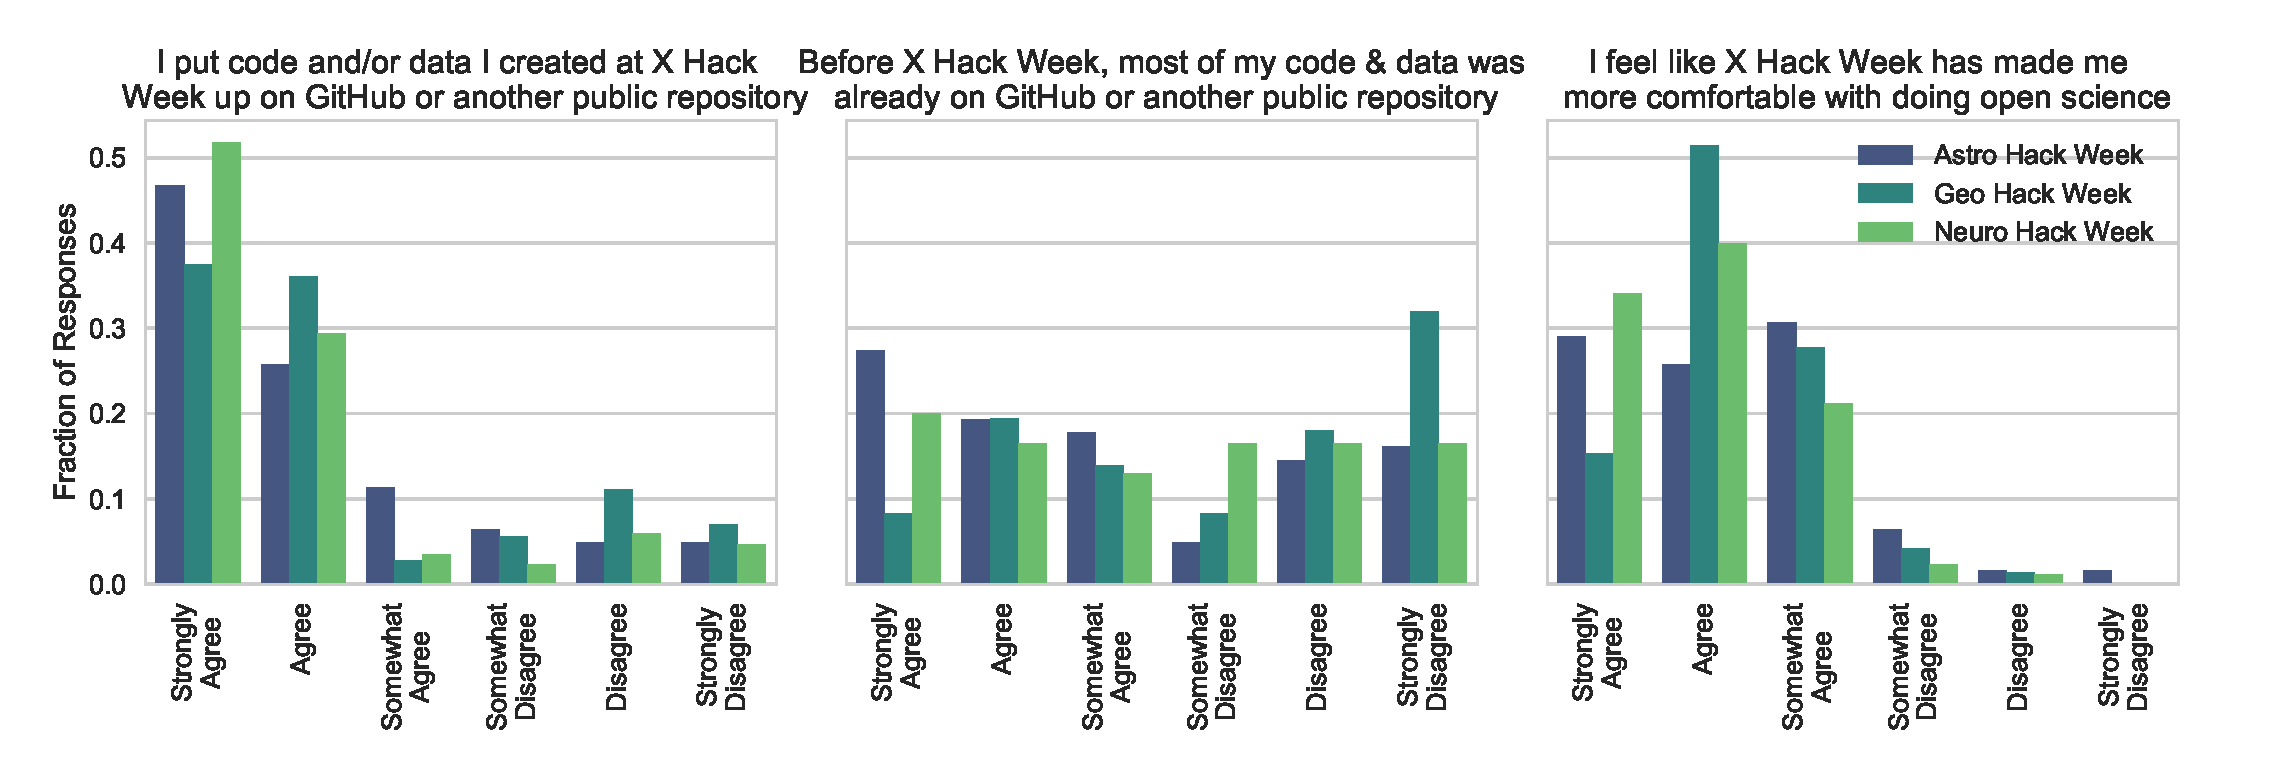
\includegraphics[width=12cm]{fig/eval_openscience}
\caption{{\bf Post-workshop surveys from three hack weeks}: participants in the 2016 astro-, geo- and neuro- hack weeks responded to questions assessing their experiences. We report here about results in three different domains: the development of technical skills (top), collaboration and learning (middle), and shifts in attitudes towards reproducibility and open science (bottom)}
\label{fig:survey}
\end{center}
\end{figure}

Because all three events are relatively recent, it is still early to evaluate long-term outcomes, such as publications and collaborations resulting from these events.
There are, however, initial indicators that all hack weeks encouraged long-term engagement with new concepts or tools and that they directly resulted in a number of publications \cite{gullysantiago2015,faria2016,keshavan2017,leonard2017,jordan2017,peterson2017,hahn2017,pricewhelan2017}. For specific examples, see also \emph{Box 1}.

\subsection{Box 1: Examples of Hack Week Outcomes}
\label{box:outcomes}
\subsubsection*{Example 1: Astro Hack Week}
In 2015, a small team used the opportunity of Astro Hack Week to found a new software project called Stingray\footnote{https://github.com/StingraySoftware/stingray} with the goal of providing well-tested, well-documented implementations of algorithms for time series analysis often used in X-ray astronomy.
The start of this project was facilitated by the collaborative environment at Astro Hack Week, including expertise in how to start/run open-source projects, role models of successful projects, and an environment encouraging scientific risk taking.
Since its beginnings at Astro Hack Week, Stingray has matured into an enduring collaboration within the community with five active maintainers, a number of contributors and four Google Summer of Code projects.
\subsubsection*{Example 2: Geo Hack Week}
In 2016, a Geo Hack Week project team used Google Earth Engine to explore spatial patterns in climate, topography and population data with the goal of mapping the most suitable locations for renewable energy sites in the United States.
The team used machine learning algorithms in conjunction with the powerful hardware resources provided by Google Earth Engine\footnote{\url{http://georgerichardson.net/2017/04/10/searching-for-energy-in-a-random-forest/}}.
George Richardson, one of the project leads, now works for a renewable resource company in Seattle.
\subsubsection*{Example 3: Neuro Hack Week}
Motion of study participants inside of the MRI machine is a major concern in neuroimaging studies.
This is a particular concern in studies in which children or patients are studied, as they are more likely to move.
In the 2016 Neuro Hack Week one of the teams focused on a large and openly available data-set of MRI data from children\footnote{ABIDE: \url{http://preprocessed-connectomes-project.org/abide}}.
To test the effect of motion on the results, the team conducted an analysis in which both the number of experimental subjects included, as well as motion cut-off were varied.
They tested both the split-half reliability of an analysis of brain connectivity, as well as an analysis that used machine learning to distinguish between brains of children with and without autism spectrum disorder.
The team (composed of four different researchers from four different institutions in two different countries) continued to work on this project remotely after the Neuro Hack Week was over, and they eventually wrote and published a paper describing these results in the open access journal Research Ideas and Outcomes \cite{leonard2017}.
